\documentclass[12pt]{article}
\usepackage{graphicx}


\begin{document}

\setlength\parindent{0pt}
\title{Raw Audio Music Generation Using Deep Neural Networks}
\author{Fabian Stahl}


\maketitle

\tableofcontents

\newpage
\section*{Abbreviations}
\begin{center}
\begin{tabular}{l l}
\textbf{CNN} & Convolutional neural network \\
\textbf{GAN} & Generative adversarial network \\
\textbf{GRU} & Gated Recurrent Unit \\
\textbf{KLD}  & Kullback–Leibler divergence\\
\textbf{LSTM} & Long short-term memory \\
\textbf{MIDI} & Musical Instrument Digital Interface \\
\textbf{MLP} & Multilayer Perceptrons \\
\textbf{RNN} & Recurrent neural network \\
\textbf{VAE} & Variational autoencoder \\
\textbf{VRNN} & Variational Recurrent neural network \\
\end{tabular}
\end{center}
\newpage


\begin{abstract}
Music can be found in almost every movie, video game or public location.
Its targeted use can change people's mood, encourage buying decisions or add context to accompanying content.
However, composing, recording and mixing music is a creative process, that takes a lot of time and skill to master.
This poses the question, if pleasing music can be generated autonomously.

Deep neural networks have been known to solve a wide range problems.
During this semester's project I will compare different network architectures to generate sample based music, show how they can be trained and rate results.
\end{abstract}

\section{Related Work}
% midi
In the field of audio generation there is a wide variety of approaches.
Most of them work with symbolic music representations, such as Ascii-text, musical scores or spectrogram data.
Especially the MIDI format is commonly used, a binary format specifying musical notes.
This makes the format very slim and easy to work with.
MIDI-based approaches include e.g. GANs with convolutions layers ~\cite{yang2017midinet, mogren2016c, mogren2016c}, VAEs paired with LSTMs~\cite{roberts2018hierarchical, tikhonov2017music, hennig2017classifying} and RNNs with restricted Boltzmann machines \cite{boulanger2012modeling}.
However, musical nuances like tonal colors, scratch and breath noises or intonations are necessary to make most music genres more interesting.
Having MIDI output only, the musical interpretation, (the raw audio sent to the sound port), is up to an external MIDI synthesizer.

There are commercial music streaming services that claim to provide generated music that fits the customer's mood.
The most prominent of them beeing brain.fm~\cite{brain.fm} and \cite{Mubert}.
However, the brain.fm algorithm only learns certain tasks, such as arrangin motifs over long timescales, while melodies, instrument choices and chord progressions are precomposed by humans.
Mubert also uses handcrafted single instrument MIDI loops, but generates some MIDI layers using decision trees, random forests and musical analysis.
Their music is limited to electronic genres only, which narrows musical variety.
While these application developers like to emphasise the machine learning aspect, their algorithms are not fully autonomous.
The two biggest reasons for that could be the high complexity of generating music sample by sample, especially with real time constraints, as well as the ineptitude of the synthesized music for commercial use.



\section{Competing Models}
\subsection{SampleRNN}
Recurrent Neural Networks (RNNs) are used to process sequences of data.
Output data is not only based upon input data, but also on a hidden state vector, that encodes previous input.
RNNs consist of arrays of small memory units.
While the original \emph{vanilla cells} were prone to the vanishing gradient problem, more advanced structures like LSTMs and GRUs could learn to keep important information and forget redundant or irrelevant previous input.
Common RNNs don't scale very good with the high temporal resolution, which is required for sound output.
Corralation can exist between neighbouring samples as well as between samples that are more than thousand frames apart.

Mehri et al. adresses this issue by using multiple stacked RNNs with different temporal resolutions (see \ref{fig::samplernn} for an example model).
Their so called \textbf{SampleRNN}~\cite{mehri2016samplernn} is a promising candidate for music generation.
Stacked \emph{Frame-Level Modules} with different fields of perception are used to capture temporal context over different time periods.
State vectors are passed to the next lower module.
A \emph{Sample-Level Module} puts their state vector into consideration as well as the current input sample to generate a probability distribution for the next sample.
Originally tested only for piano music, \cite{zukowski2018generating} and \cite{carr2018generating} showed, that SampleRNN is especially good to generate loud music genres, like Metal and Dark Ambient.
Its biggest drawback is, that sample quality varies strongly even after days of training.




\subsubsection{Architecture}
\begin{figure}[ht]
    \label{fig:samplernn}
    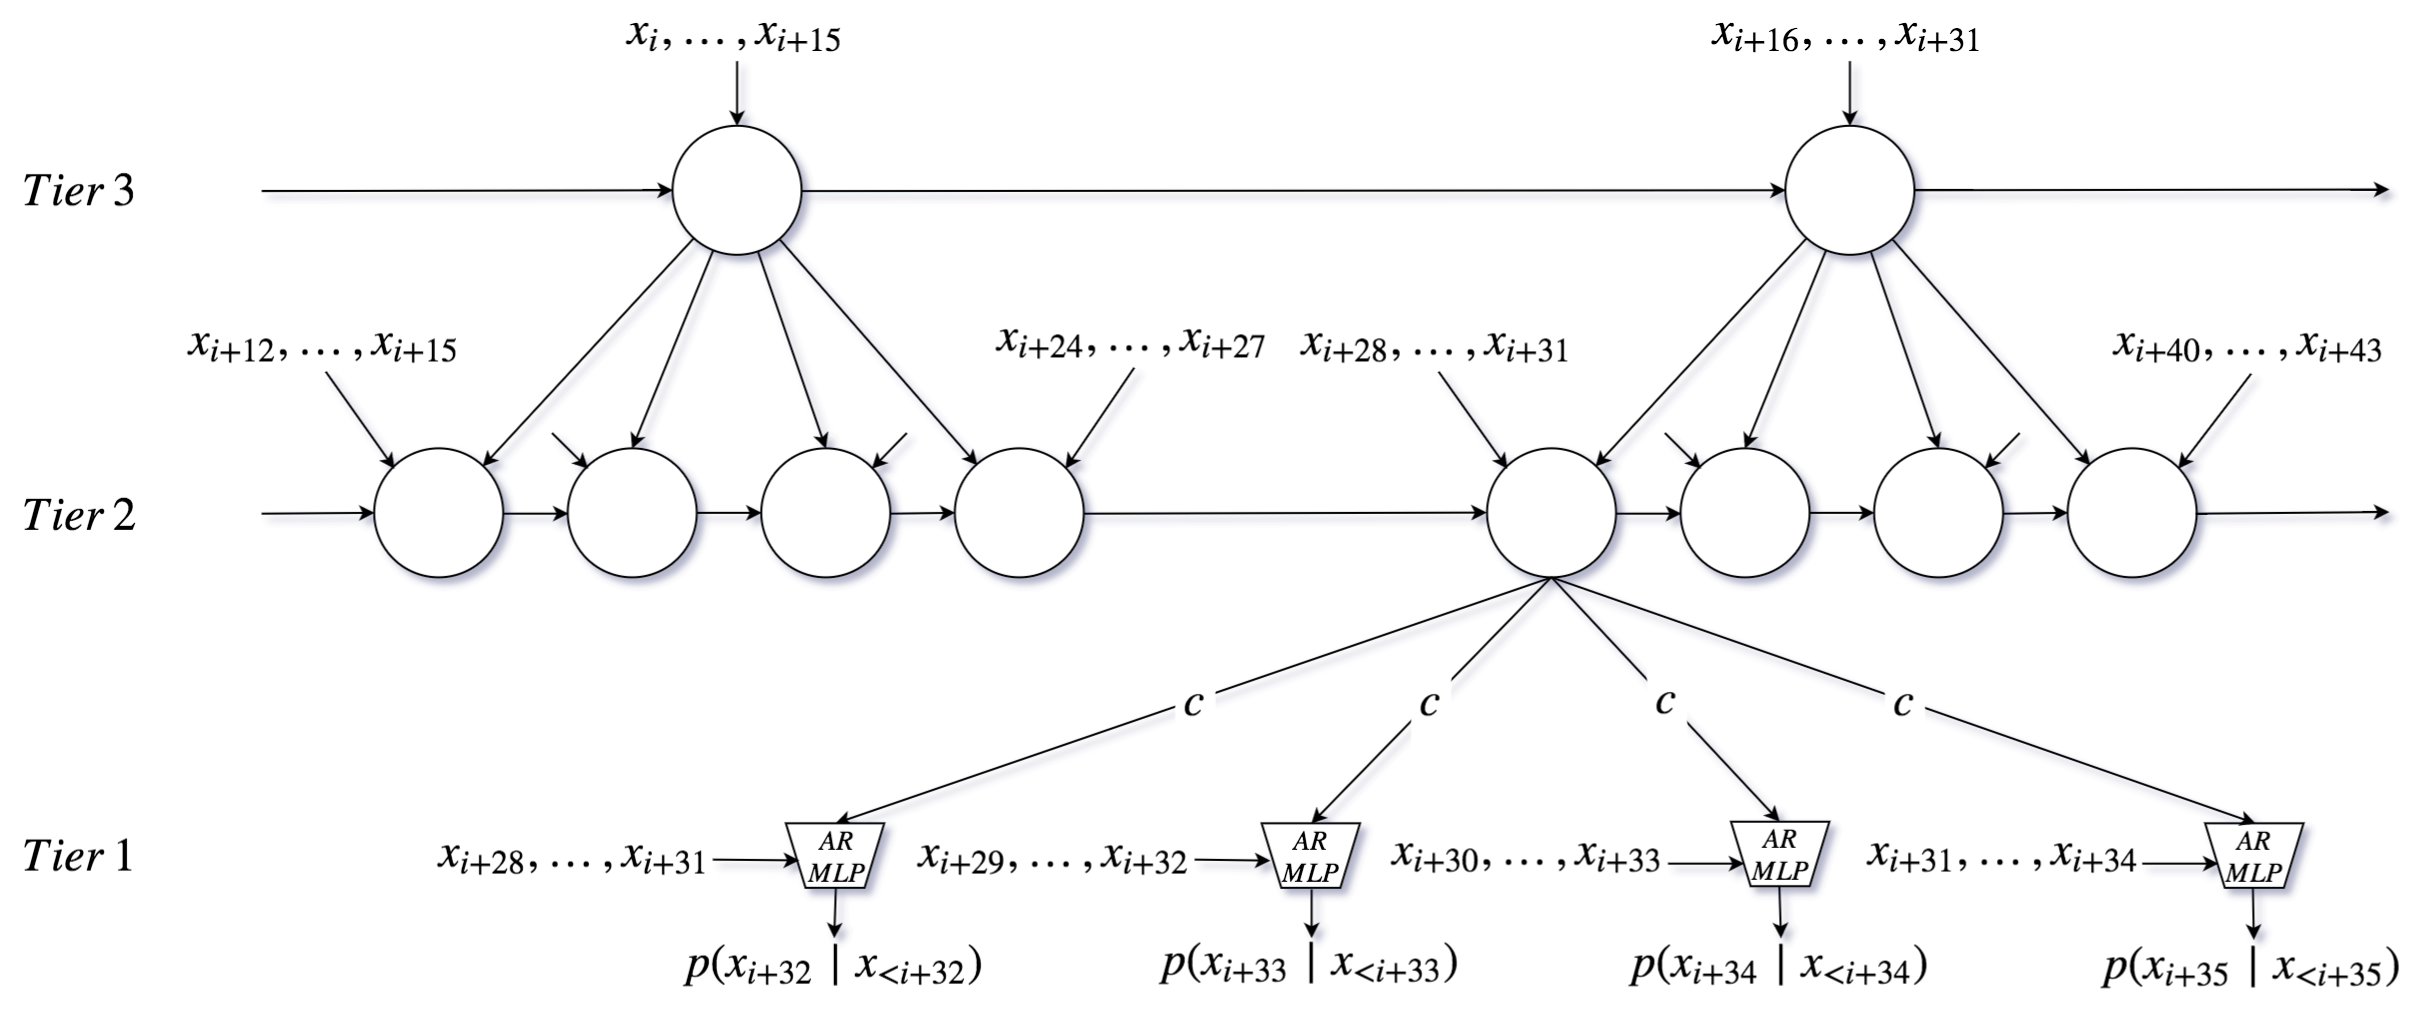
\includegraphics[width=\textwidth]{img/samplernn.png}
    \caption{The SampleRNN consist of multiple Frame-Level Modules, two in this example, and a Sample-Level Module (tier 1). Here, tier 3 has a field of perception of 15 samples, whereas tier 2 uses 3 samples each step and needs to be called more frequently. The state vector $c$ of tier 3 is passed to tier 2 and combined with its state vector $h$. Tier 1 takes the product of $c$ and the sample input and feeds it trough a MLP to determine a probability distribution to draw the next sample. Note that this example is simplified. }
\end{figure}

\subsubsection{Experiments}

\subsection{VRNN}

 % Paper
\cite{VRNNgit} % Implementation

% Idee (Markov, variational autoencoder erklären)

Another approach to generate sound data is the Variational Recurrent Neural Network (VRNN), proposed 2016 by Chung et al.~\cite{chung2015recurrent}.
The architecture was trained on the tasks of handwriting and sound generation.
However, experiments for the ladder only include training with speech datasets and non-linguistic human-made sounds like coughing and screaming.
This poses the question if the VRNN can be used to generate music as well.

Chung et al. states, that there is an issue in the way that RNNs model output variety, since the only source of true randomness is drawing values from an output probability density.
Data that is both highly variable and highly structered can be hard to model this way.
On the one hand small input variations should lead to potentially very large variations in the hidden state vector $h_t$, on the other hand, different high level structures need to be mapped to distinct state vectors as well.
This forces the network to compromise the encoding of low-level and high-level features.
The main idea of the VRNN is to extend a recurrent neural network with latent random variables, therefore improving the representational power of the model.
Such high-level variables are commonly used in VAEs to model multimodal conditional distributions, approximating real world data variety~\cite{kingma2013auto}.
% <Satz zu VAEs>
Chung et al. proposes to extend the VEA model by inducing temporal dependencies using the hidden state vector of a RNN across neighboring timesteps.




% Architektur erklären (Diagramme, Fehlerfunktionen, Trainingsdiagramme)



% Describe p, q, ...

conditional prior / generative model - p(x | z)

variational approximation 
approximate posterior / inference model - p(z | x)
prior over latent random variables - p(z)



The model can be trained by minimizing the Kullback–Leibler divergence (KLD) - first term - and maximizing the likelihood of an $x$ given a $z$ - second term).
This can be seen as adding a regulizer to a simple auto encoder to ensure that the generated distributions have a certain form.
$$
E_{\mathbf{z} \le T | \mathbf{x} \le T} = \left[ \sum_{t=1}^T -(KL(q(\mathbf{z}_t | \mathbf{x}_{\le t}, \mathbf{z}_{<t}) || p(\mathbf{z}_t | \mathbf{x}_{<t}, \mathbf{z}_{<t})) + log(p(\mathbf{x}_t | \mathbf{z}_{\le t, \mathbf{x}_{<t}}))) \right]
$$

The KLD between the two distributions $Q$ and $P$ with respect to $Q$ can be seen as a measurment of similarity between two distributions \cite{}.
Since the probabilistic Encoder $q(z|x)$ is used to approximate the hard to compute posterior $p(x|z)$, $Q$ needs to be as similar to $P$ as possible.
This means that the KL divergence needs to be minimized, which is identical to maximizing the lower variational bound~\cite{kingma2013auto}.
%The KLD is defined as:
%$$
%KL(q || p) = -\sum p(x) log(\frac{p(x)}{q(x)})  
%$$

The second term of the error function describes the reconstruction error.
%$$
%log p(\mathbf{x}_t | \mathbf{z}_{\le t, \mathbf{x}_{<t}})
%$$

In theory the model can be trained using any probability distribution.
The original paper uses gaussian distributions, leading to
$$
KL(q(\mathbf{z}_t | \mathbf{x}_{\le t}, \mathbf{z}_{<t}) || p(\mathbf{z}_t | \mathbf{x}_{<t}, \mathbf{z}_{<t}))
= \sum \frac{log(\sigma_2)}{log(\sigma_1)}+\frac{\sigma_1^2 + (\mu_1 - \mu_2)}{2 \sigma_2^2} - \frac{1}{2}
$$
for term 1, where $\mu_1$ and $\mu_2$ are mean values and $\sigma_1$ and $\sigma_2$ are are the standard deviations of the two distributions $p$ and $q$ (see \cite{klproof} for a proof ), and
$$
log(p(\mathbf{x}_t | \mathbf{z}_{\le t, \mathbf{x}_{<t}}))
= \sum \frac{\sqrt{y-\mu}}{2 \sigma^2} + log(\sigma) + \frac{log(2\pi)}{2}
$$
describes the second term, where %To_do!


% Implementierungsdetaills
Since the original source code was using the Theano ML library, I cloned a public PyTorch implementation~\cite{VRNNgit}.
However, I found out, that I needed to make quite many adaptions to fit the original version.
The biggest changes include a new data loader class, adding the correct error function, using more dense layers in all components and make the code more GPU-friendly.


% Results

\subsubsection{Architecture}
\subsubsection{Training}

\subsection{???}
\subsubsection{Architecture}
\subsubsection{Training}

\section{Evaluation}
\subsection{Challenges}
\subsection{Performance}
\subsection{Comparison to Real Music}
\subsection{Human Evaluation}

\section{Discussion and future work}





\end{document}
